\section{Mise en \oe{}uvre}

\begin{frame}
\tableofcontents[currentsection, hideothersubsections]
\end{frame}

\subsection{Grapher}
\begin{frame}{Grapher}
\begin{center}
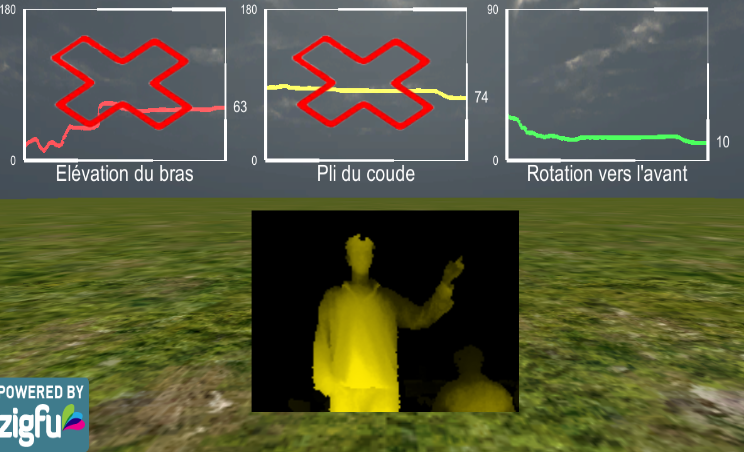
\includegraphics[width=0.9\linewidth]{../images/zfm_graph}
\end{center}
\end{frame}

\subsection{Multi Cameras}
\begin{frame}{Multi Cameras}
\begin{center}
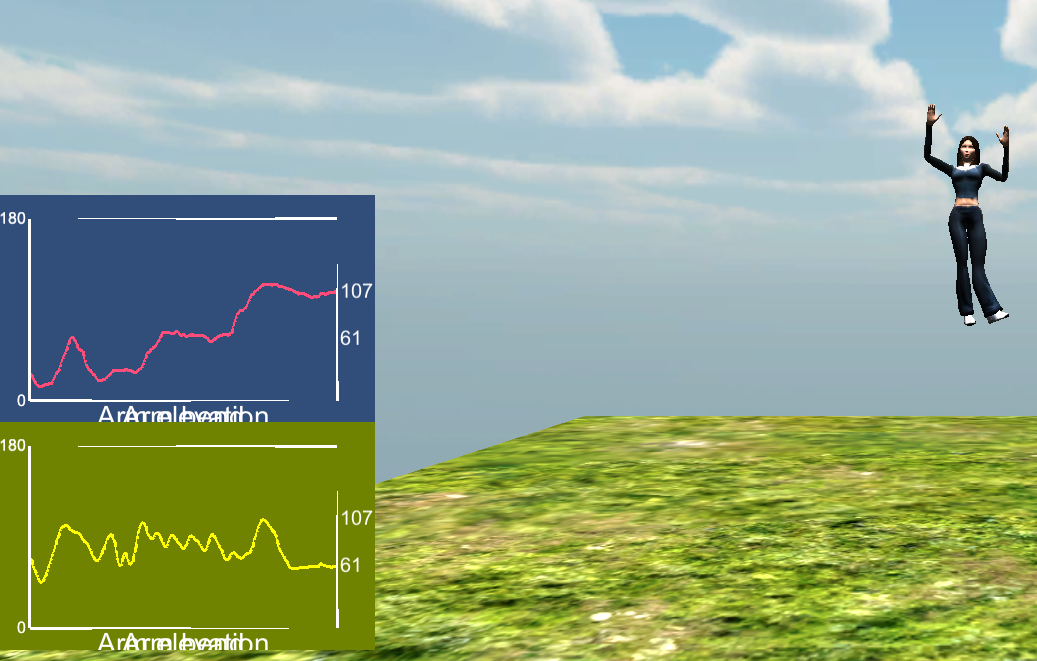
\includegraphics[width=0.9\linewidth]{../images/multicamera}
\end{center}
\end{frame}

\subsection{Avatar 3D}
\begin{frame}{Avatar 3D}
\begin{center}
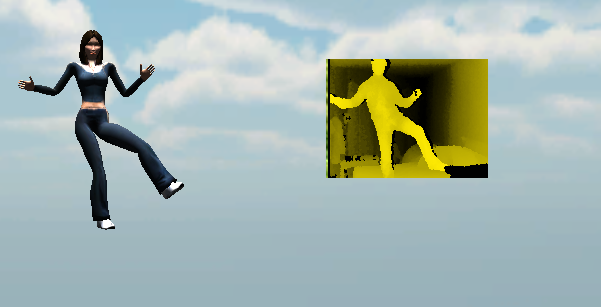
\includegraphics[width=0.9\linewidth]{../images/avatar3D}
\end{center}
\end{frame}

\subsection{Menus}
\begin{frame}{Menus}
\begin{center}
\only<1>{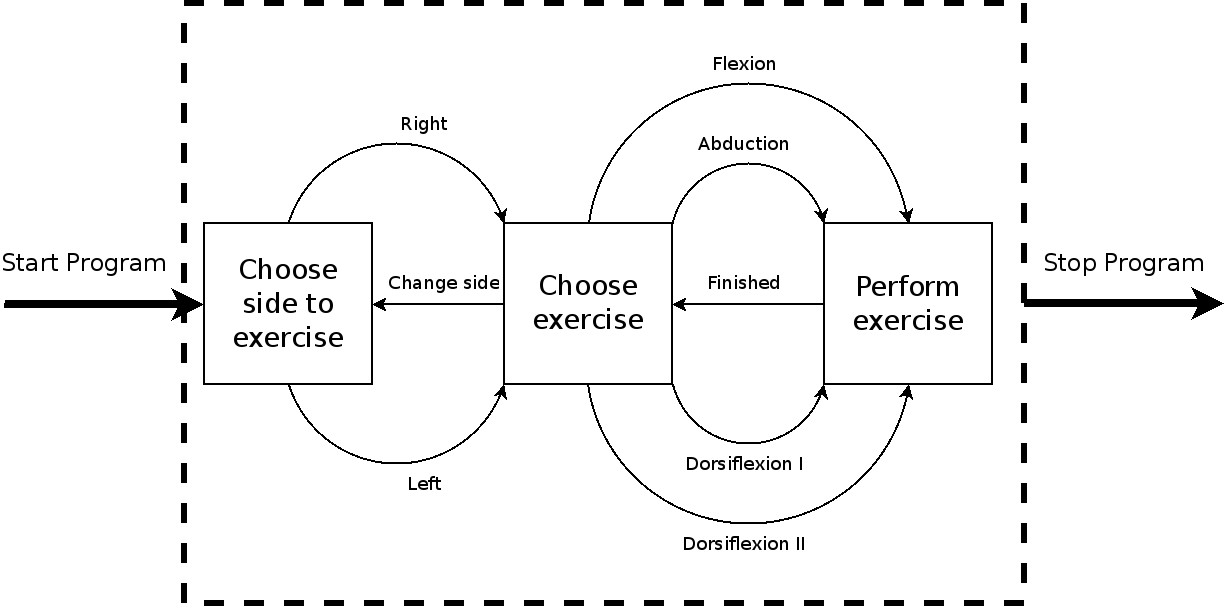
\includegraphics[width=1.0\linewidth]{../images/menu}}
\only<2>{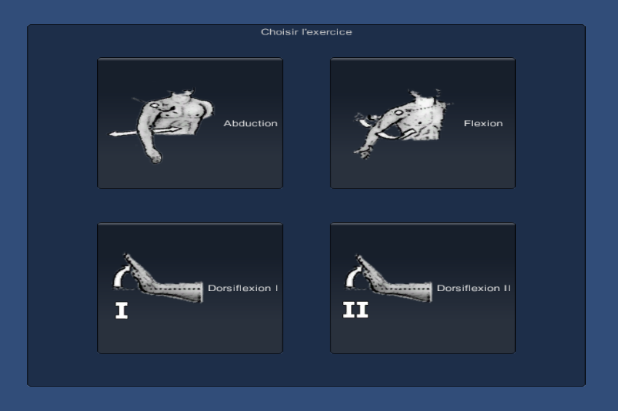
\includegraphics[width=0.8\linewidth]{../images/menu2}}
\end{center}
\end{frame}

\subsection{ExerciseMonitor}
\begin{frame}{Menus}
\begin{center}
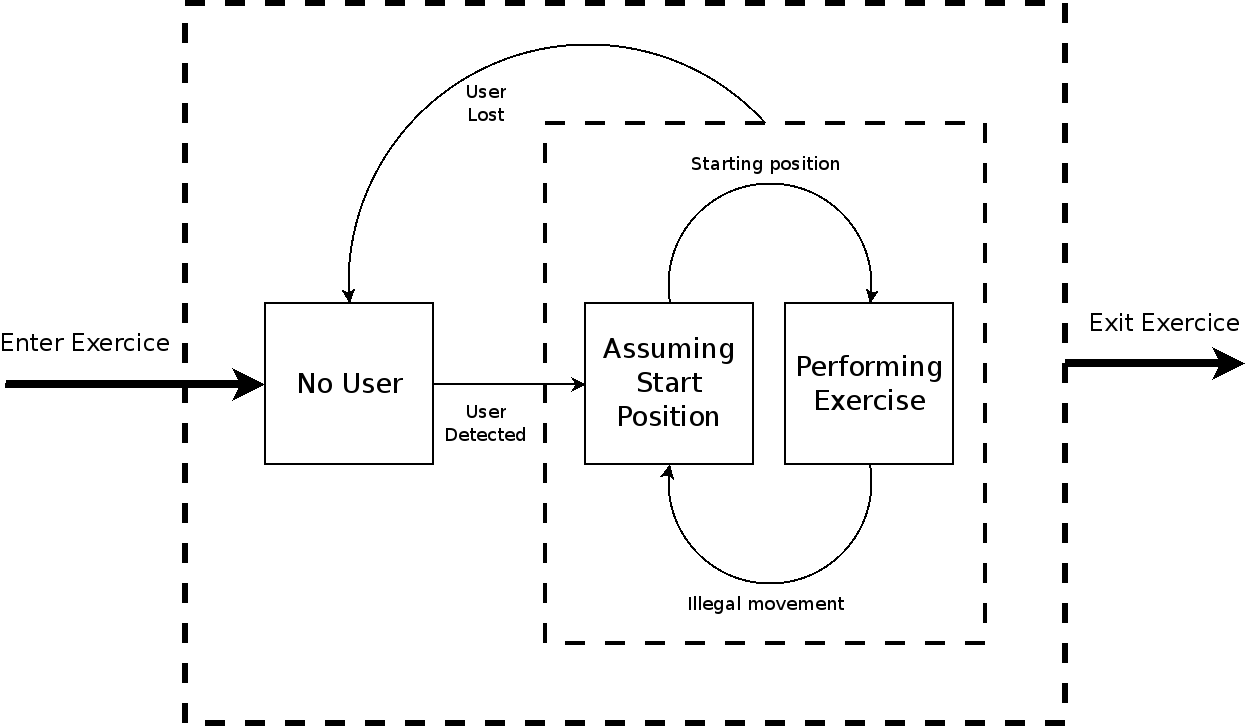
\includegraphics[width=1.0\linewidth]{../images/exercise_monitor}
\end{center}
\end{frame}

\subsection{À posteriori}
\begin{frame}{À posteriori}
\only<1-2>
{
  \begin{block}{Résultats}
  \begin{itemize}
  \item Test automatique,
  \item Retour granulaire,
  \item Aspect ludique qui émerge du retour d'informations.
  \end{itemize}
  \end{block}
}
\only<2>
{
  \begin{alertblock}{Problèmes}
  \begin{itemize}
  \item Trop de temps passé dans les menus,
  \item Le patient regarde le membre,
  \item Le retour incite à forcer.
  \end{itemize}
  \end{alertblock}
}
\only<3-4>
{
  \begin{alertblock}{Limites}
  \begin{itemize}
  \item Précision insuffisante,
  \item Pas de mesure des rotations,
  \item Zigfu.
  \end{itemize}
  \end{alertblock}
}
\only<4>
{
  \begin{block}{Ouverture}
  \begin{itemize}
  \item Poursuite de l'étude en stage~:
  \begin{itemize}
  \item \textbf{Geoffrey~:} aspects ludiques, difficulté dynamique,
  \item \textbf{William~:} meilleur extraction de squelette. 
  \end{itemize}
  \end{itemize}
  \end{block}
}

\end{frame}